%%
%% The acknowledgments section is defined using the "acks" environment
%% (and NOT an unnumbered section). This ensures the proper
%% identification of the section in the article metadata, and the
%% consistent spelling of the heading.

% \begin{acks}
% Lorem ipsum dolor sit amet, consectetur adipiscing elit.
% \end{acks}

%%
%% The next two lines define the bibliography style to be used, and
%% the bibliography file.
\bibliographystyle{ACM-Reference-Format}
\bibliography{report}

%%
%% If your work has an appendix, this is the place to put it.
\appendix

\section{Ban Lift Analysis}
\label{appendix:banlift}

To further examine the causal relationship and strengthen our interpretation, we analyze the period following the ban's lift on April 28, 2023. This analysis serves as a complementary test of our circumvention hypothesis: if Italian developers experienced a genuine productivity decline during the ban (due to inability to access ChatGPT), we would expect to observe a positive rebound effect when access was officially restored. Conversely, if developers successfully circumvented the ban and maintained access throughout the restriction period, the official lifting should have no effect—they would already be using ChatGPT regardless of its legal status. This logic provides a powerful test of whether the ban was effectively enforced or circumvented.

Table~\ref{tab:did-lift} presents difference-in-differences estimates comparing coding activity before and after the ban was lifted, using the same time windows as our main analysis. The coefficient on ``Italy × Post-Lift'' represents whether developers in Italy experienced a rebound in coding activity relative to the control countries once ChatGPT access was officially restored.

\begin{table}[htbp]
  \centering
  \caption{Difference-in-Differences Results: Post-Ban Lift (Absorbed Fixed Effects)}
  \label{tab:did-lift}
  \begin{table}[!htbp] \centering
  \caption{Difference-in-Differences Estimates: Lines of Code Changes After ChatGPT Ban Lift}
  \label{tab:did-lift}
\begin{tabular}{@{\extracolsep{5pt}}lcccc}
\\[-1.8ex]\hline
\hline \\[-1.8ex]
\\[-1.8ex] & \multicolumn{1}{c}{LOC Added (2 Weeks)} & \multicolumn{1}{c}{LOC Added (4 Weekdays)} & \multicolumn{1}{c}{LOC Deleted (2 Weeks)} & \multicolumn{1}{c}{LOC Deleted (4 Weekdays)}  \\
\hline \\[-1.8ex]
 Italy & -4086.519$^{}$ & -4010.950$^{}$ & -1077.617$^{}$ & -1231.823$^{}$ \\
& (5620.952) & (5770.782) & (1337.319) & (1315.548) \\
 Post-Lift & -1055.302$^{}$ & 566.091$^{}$ & 625.877$^{}$ & 1660.161$^{}$ \\
& (1685.454) & (2932.394) & (1173.611) & (1880.063) \\
 Italy × Post-Lift & 643.460$^{}$ & -2767.974$^{}$ & 258.638$^{}$ & -904.240$^{}$ \\
& (2735.654) & (3758.932) & (2029.785) & (2714.440) \\
 Constant & 16726.655$^{***}$ & 17113.333$^{***}$ & 6773.386$^{***}$ & 7076.681$^{***}$ \\
& (4418.021) & (4613.066) & (894.855) & (929.972) \\
\hline \\[-1.8ex]
 Observations & 209142 & 169574 & 209142 & 169574 \\
 $R^2$ & 0.000 & 0.000 & 0.000 & 0.000 \\
 Adjusted $R^2$ & 0.000 & 0.000 & -0.000 & -0.000 \\
 Residual Std. Error & 378708.112 (df=209132) & 390728.730 (df=169564) & 190160.556 (df=209132) & 197850.531 (df=169564) \\
 F Statistic & 0.616$^{}$ (df=9; 209132) & 0.691$^{}$ (df=9; 169564) & 0.714$^{}$ (df=9; 209132) & 1.561$^{}$ (df=9; 169564) \\
\hline
\hline \\[-1.8ex]
\textit{Note:} & \multicolumn{4}{r}{$^{*}$p$<$0.1; $^{**}$p$<$0.05; $^{***}$p$<$0.01} \\
\end{tabular}
\end{table}

  \par\vspace{0.1cm}
  \textit{Notes:} Absorbed fixed effects for users and dates. Robust standard errors are clustered on the user-level in parentheses. *** p$<$0.01, ** p$<$0.05, * p$<$0.1
\end{table}

We find no statistically significant effects in any of the specifications. For the two-week post-lift period, the treatment effects are -0.0321 (SE: 0.0494) for log additions and -0.0044 (SE: 0.0502) for log deletions. For the four-weekday period, the effects are -0.0158 (SE: 0.0541) and -0.0585 (SE: 0.0547), respectively. All coefficients are small in magnitude, not statistically significant, and show no consistent pattern of positive rebound. 

The absence of any observable increase in coding activity following the ban's lift is consistent with our main interpretation: developers had already restored access through circumvention (primarily VPNs, as documented in Appendix~\ref{appendix:circumvention}) weeks before the official lifting. If they were already using ChatGPT throughout the ban period, the legal change on April 28 would have no marginal impact on their actual access or productivity—which is precisely what we observe. This null result, combined with the null finding during the ban period itself, provides mutually reinforcing evidence that the treatment was effectively porous due to widespread circumvention.

\section{Ban Circumvention Analysis}
\label{appendix:circumvention}

This appendix presents the difference-in-differences analysis of search volume for circumvention tools---specifically VPN services and Tor Browser---in Italy (treatment group) compared to Austria and Germany (control groups) before and after the ban implementation on April 1st, 2023. The data was obtained from Google Trends~\cite{googletrends}, which provides normalized search interest values representing the share of web searches for a given term relative to all searches on Google over time. The values are normalized on a scale of 0--100, where 100 represents peak popularity for the term during the selected time period.

Figure~\ref{fig:vpn-timeseries} shows the VPN search volume over time for Italy, Austria, and Germany. The vertical dashed line indicates the ban start date (April 1st, 2023). Prior to the ban, Italy showed consistently lower baseline search interest in VPNs compared to the control countries, with average values around 21 points versus 33--35 points for Austria and Germany. Following the ban implementation, Italy experienced a dramatic spike in VPN search interest, reaching a peak of 100 (the maximum normalized value) on April 1st, and maintaining elevated levels throughout the post-ban period with an average of 51 points.

\begin{figure}[htbp]
\centering
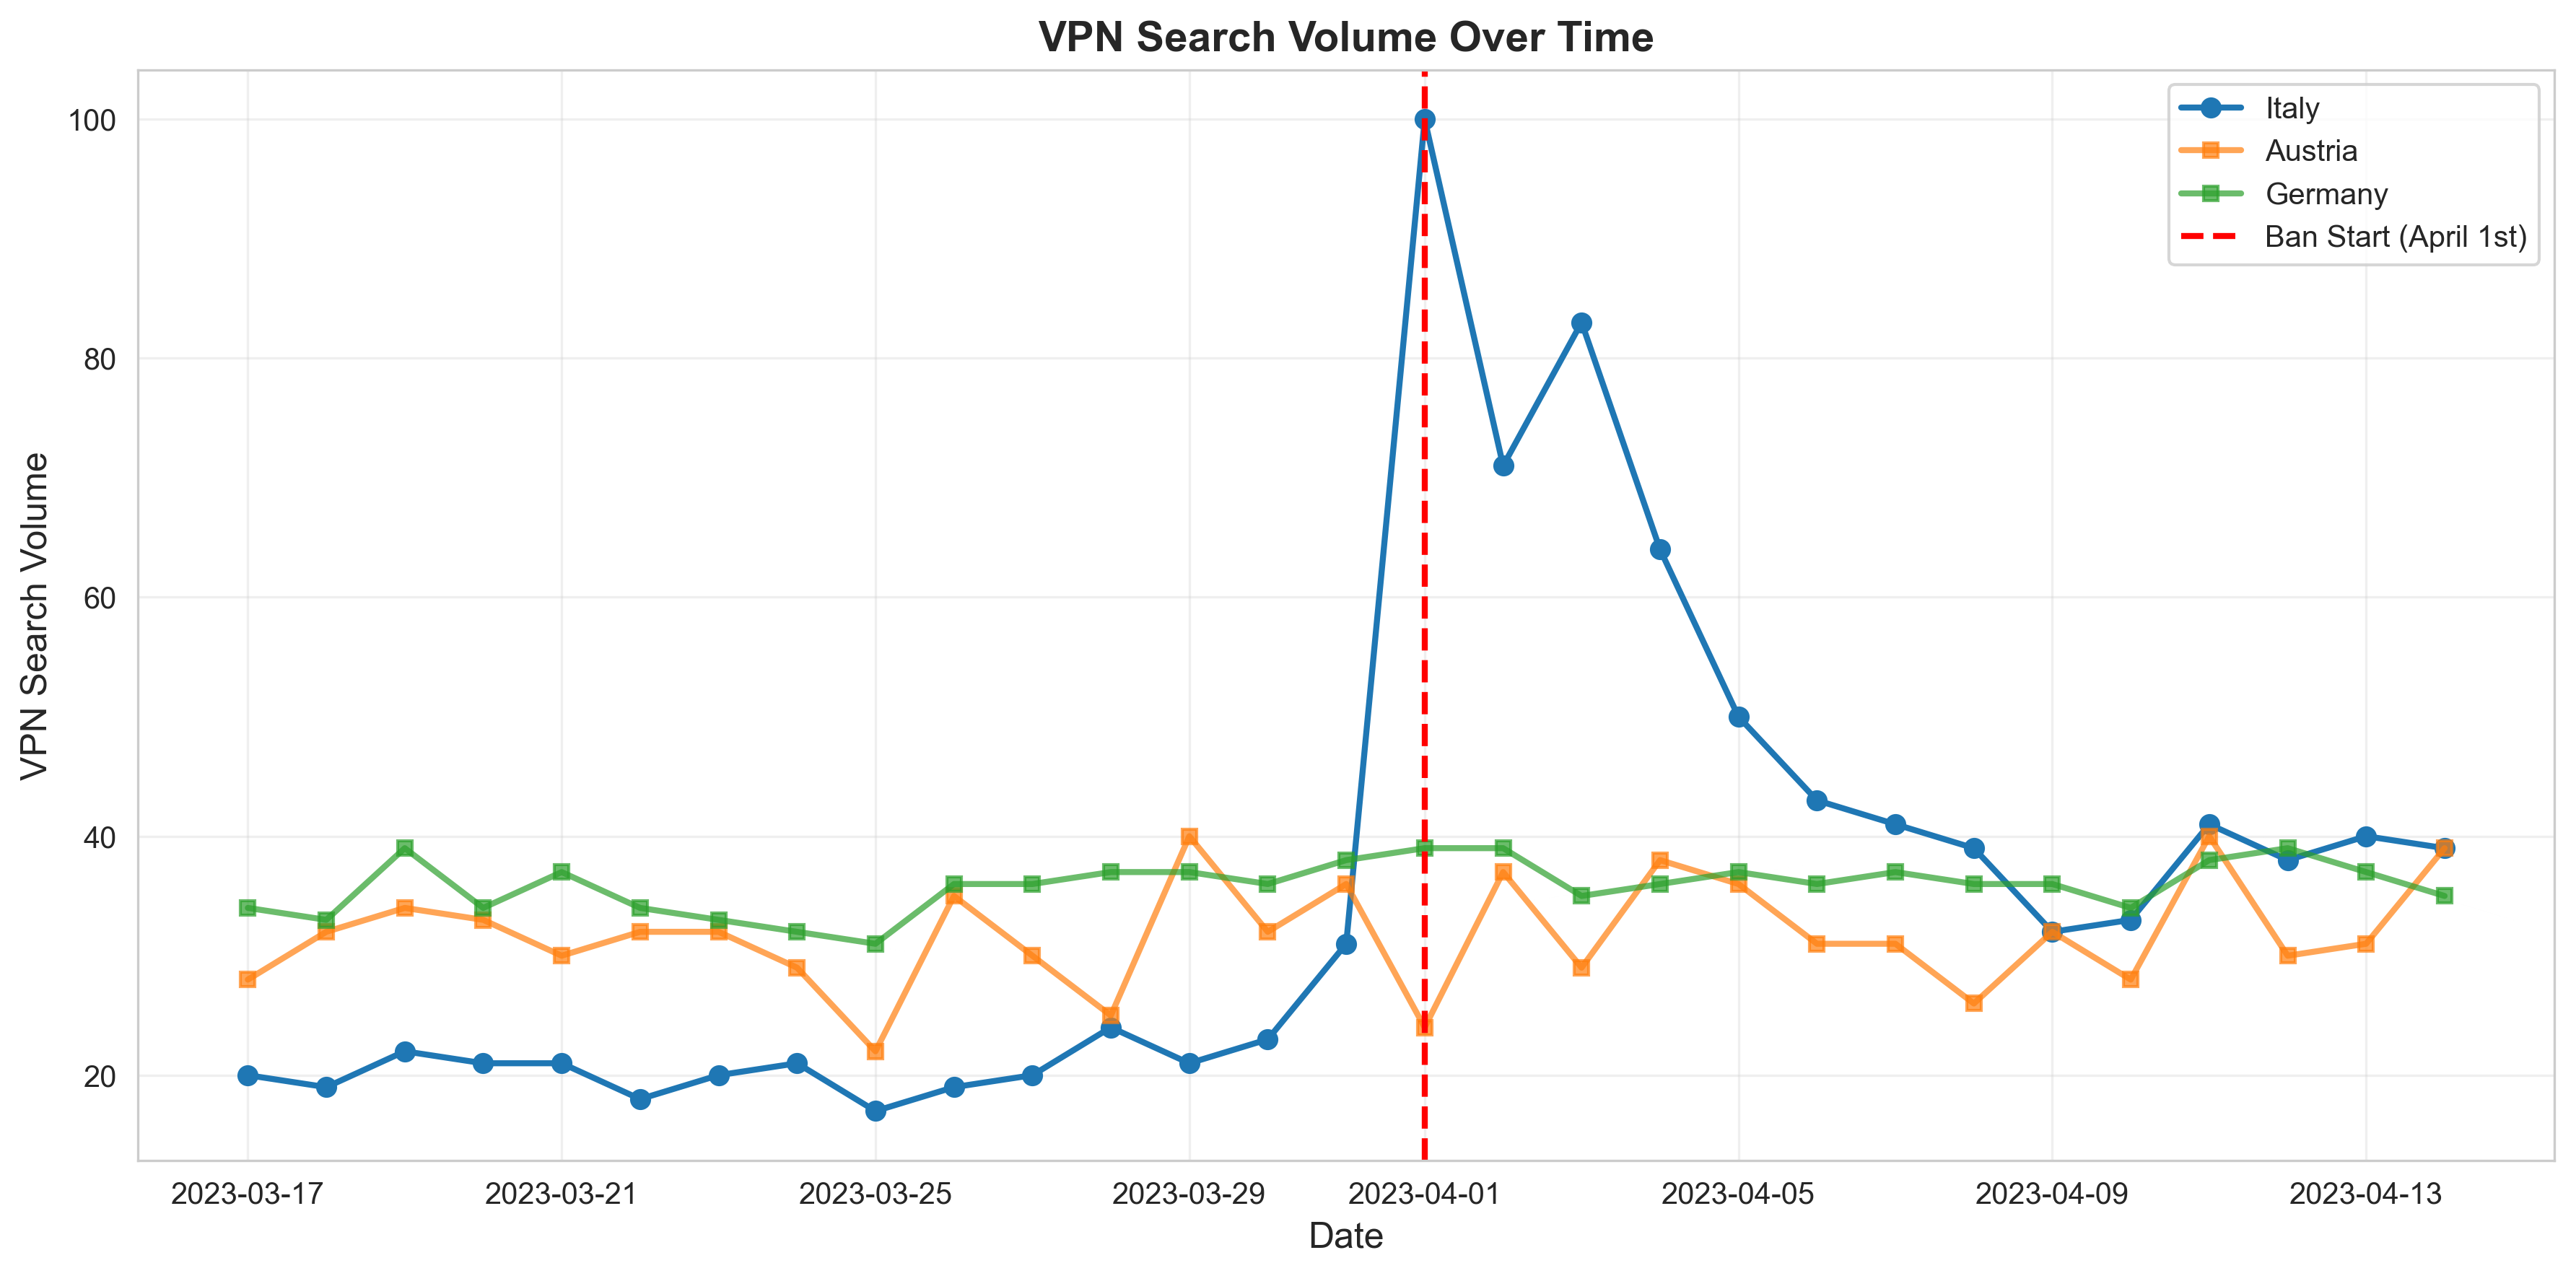
\includegraphics[width=0.9\textwidth]{../Google Search DiD/did_vpn_timeseries_plot.png}
\caption{VPN Search Volume Over Time}
\label{fig:vpn-timeseries}
\end{figure}

Figure~\ref{fig:vpn-before-after} compares the average VPN search volume before and after the ban implementation across the three countries. The visualization clearly demonstrates the substantial increase in VPN search interest in Italy following the ban, while the control countries (Austria and Germany) showed minimal changes, consistent with the parallel trends assumption required for difference-in-differences estimation.

\begin{figure}[htbp]
\centering
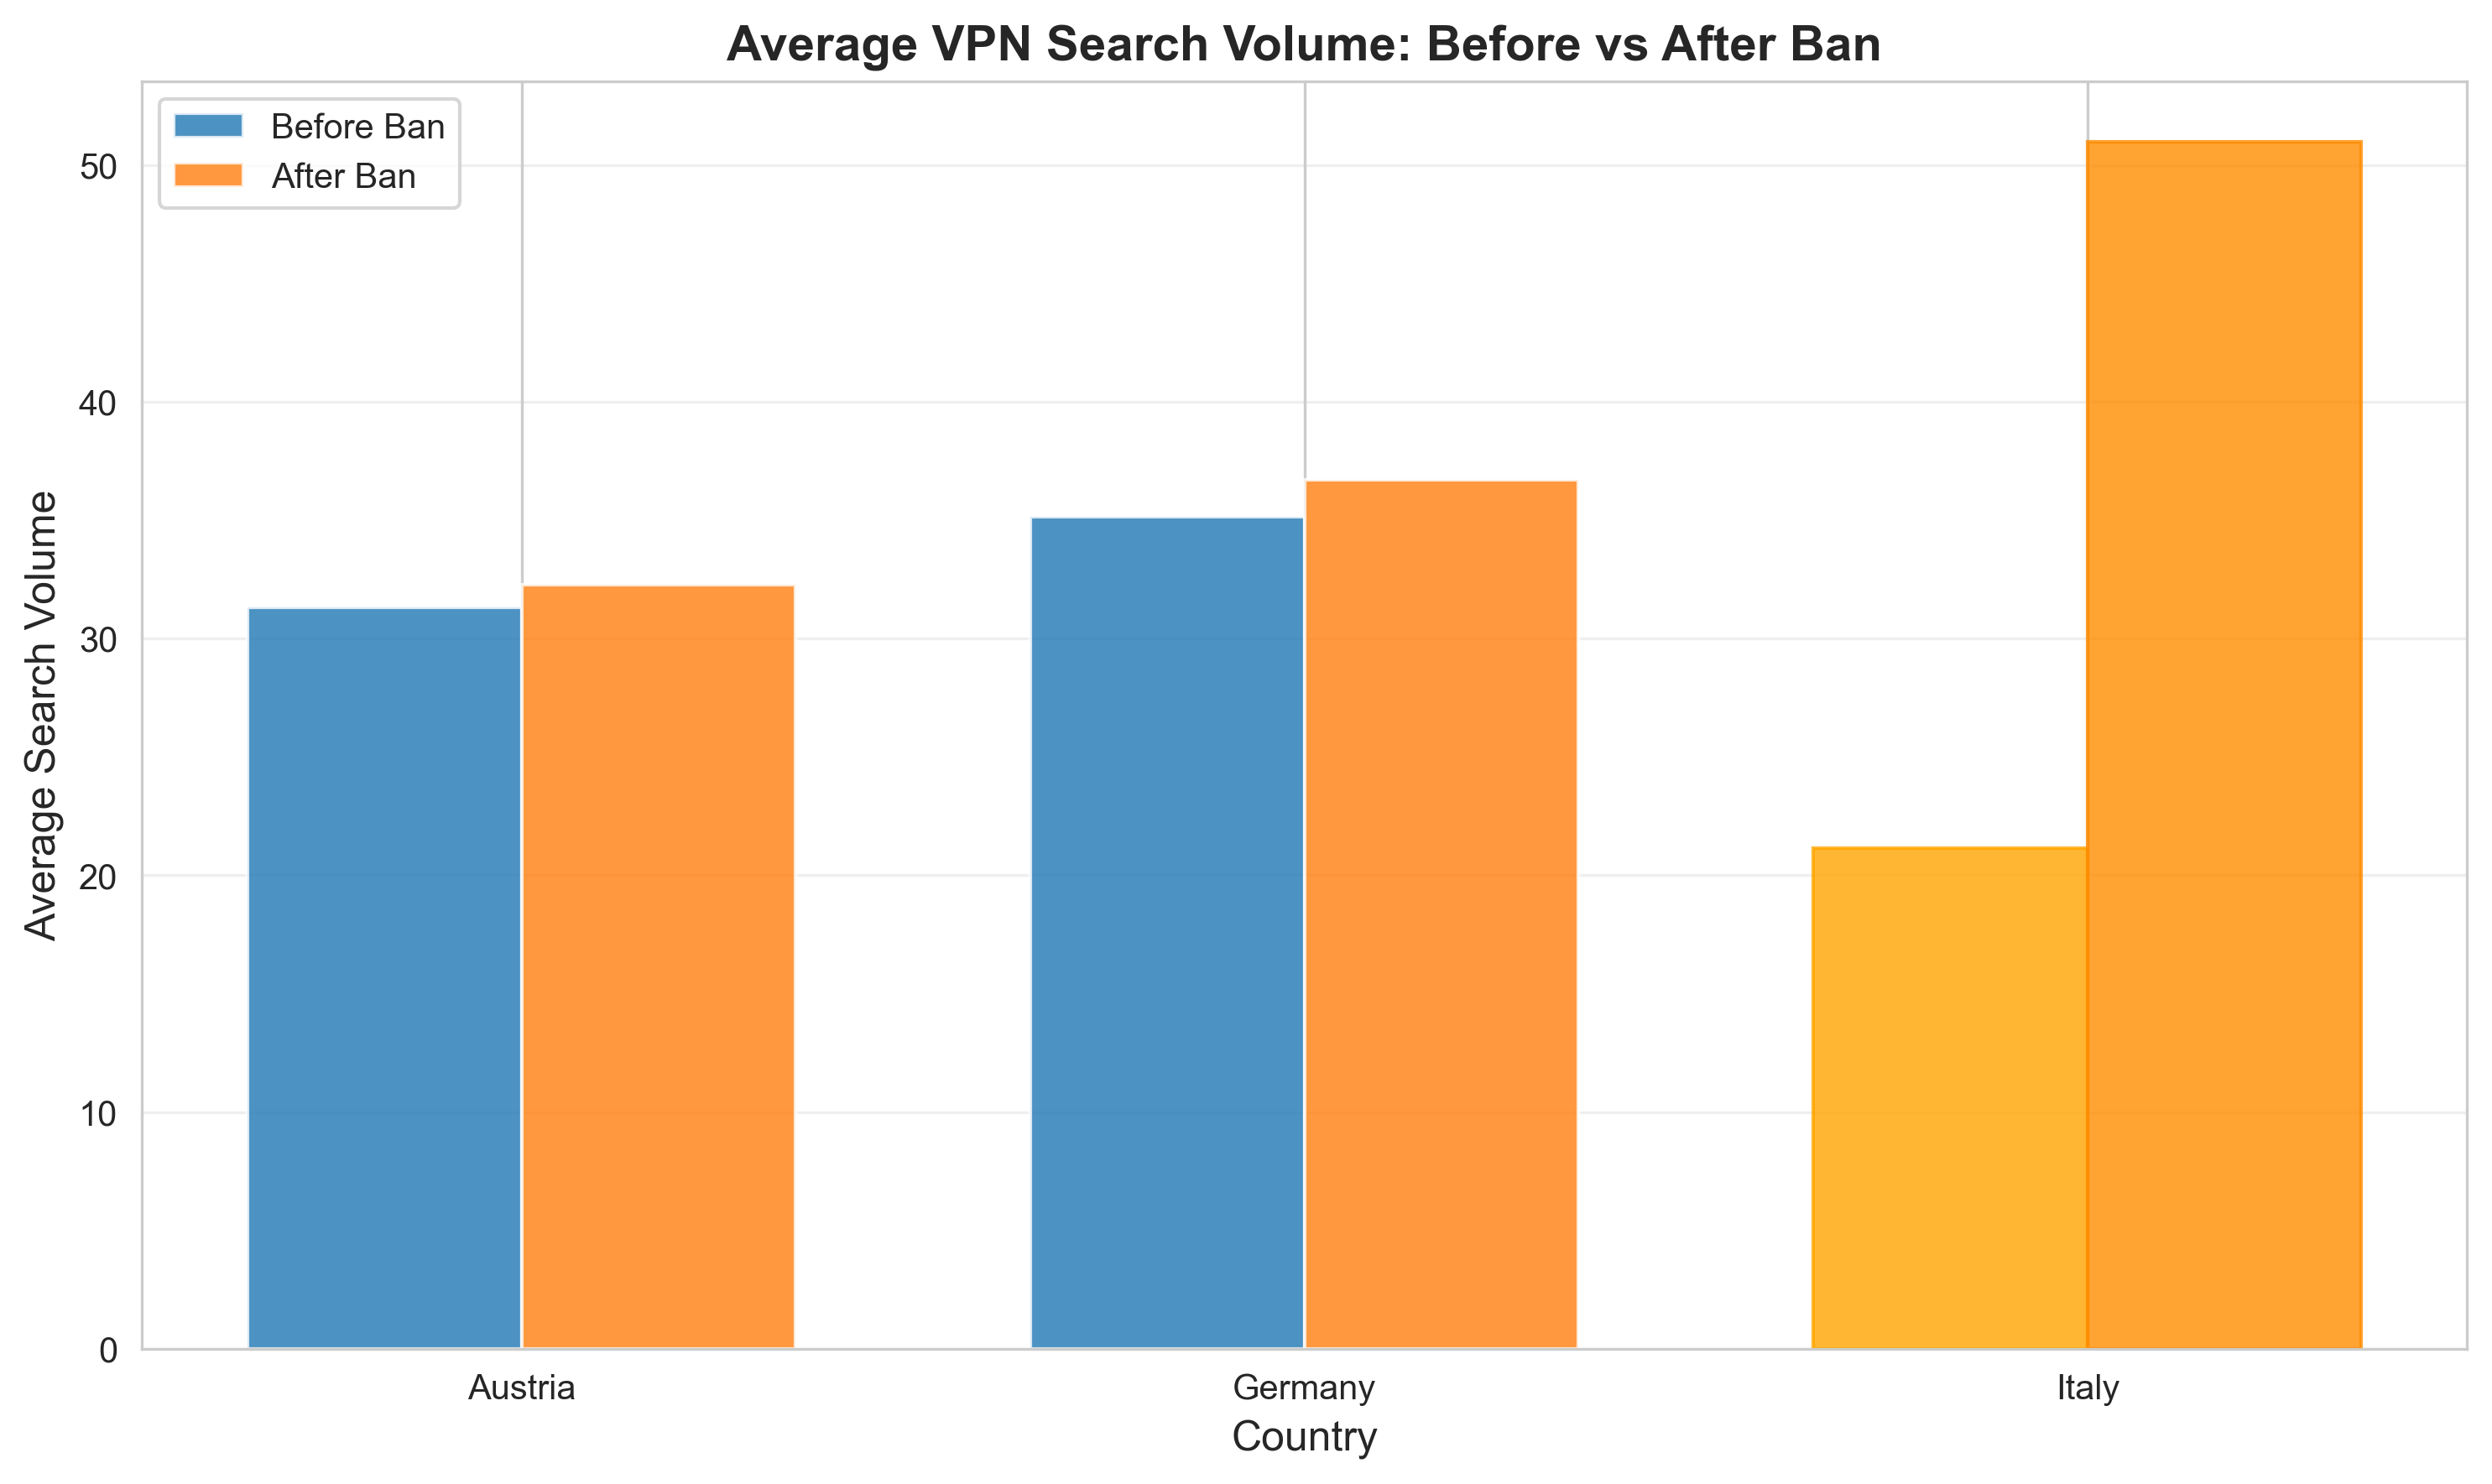
\includegraphics[width=0.8\textwidth]{../Google Search DiD/did_vpn_before_after_plot.png}
\caption{Average VPN Search Volume: Before vs After Ban}
\label{fig:vpn-before-after}
\end{figure}

Table~\ref{tab:circumvention-regression} presents the difference-in-differences regression results for both VPN and Tor Browser searches. The dependent variable in each model is search volume (normalized Google Trends index). The coefficient on ``Italy × Post-Ban'' represents the treatment effect for each circumvention tool. For VPN searches, the coefficient indicates that searches in Italy increased by 28.6 points (on the 0--100 scale) more than in the control countries after the ban implementation, an effect that is statistically significant at the 1\% level ($p < 0.001$). For Tor Browser searches, the treatment effect is 20.2 points, statistically significant at the 5\% level ($p < 0.05$). These results suggest a substantial increase in interest in both VPN services and Tor Browser as means of circumventing the ban. The magnitude of the VPN effect represents more than a doubling of baseline search interest in Italy, consistent with users seeking tools to bypass geographic restrictions.

\begin{table}[htbp]
\centering
\caption{Difference-in-Differences Regression Results}
\label{tab:circumvention-regression}
\begin{tabular}{@{\extracolsep{5pt}}lcc}
\\[-1.8ex]\hline
\hline \\[-1.8ex]
& \multicolumn{2}{c}{\textit{Dependent variable: search\_volume}} \
\cr \cline{2-3}
\\[-1.8ex] & \multicolumn{1}{c}{VPN} & \multicolumn{1}{c}{Tor Browser}  \\
\hline \\[-1.8ex]
 Italy & -12.100$^{***}$ & -10.167$^{}$ \\
& (2.823) & (6.221) \\
 Post-Ban & 1.267$^{}$ & -0.710$^{}$ \\
& (2.346) & (5.169) \\
 Italy × Post-Ban & 28.600$^{***}$ & 20.167$^{**}$ \\
& (4.063) & (8.953) \\
 Constant & 33.233$^{***}$ & 17.567$^{***}$ \\
& (1.630) & (3.592) \\
\hline \\[-1.8ex]
 Observations & 87 & 87 \\
 $R^2$ & 0.497 & 0.079 \\
 Adjusted $R^2$ & 0.479 & 0.046 \\
 Residual Std. Error & 8.928 (df=83) & 19.672 (df=83) \\
 F Statistic & 27.344$^{***}$ (df=3; 83) & 2.371$^{*}$ (df=3; 83) \\
\hline
\hline \\[-1.8ex]
\textit{Note:} & \multicolumn{2}{r}{$^{*}$p$<$0.1; $^{**}$p$<$0.05; $^{***}$p$<$0.01} \\
\end{tabular}
\end{table}
